\documentclass[../Languages.tex]{subfiles}

\begin{document}
\usec{Perl}\label{sec:perl}

\cd{Perl} is a family of high-level, general-purpose, interpreted, dynamic
programming language. The languages in this family include \cd{Perl 5} and
\cd{Perl 6}.

Though \cd{Perl} is not officially an acronym, there are various backronyms in
use, including ``Practical Extraction and Reporting Language''. \cd{Perl} was
originally developed by Larry Wall in 1987 as a general-purpose Unix scripting
language to make report processing easier. Since then, it has undergone many
changes and revisions. \cd{Perl 6} which began as a redesign of \cd{Perl 5} in
2000, eventually evolved into a separate language. Both languages continue to
be developed independently by different development teams and liberally borrow
ideas from one another.

The \cd{Perl} languages borrow features from other programming languages
including \cd{C}, \cd{sh}, \cd{AWK}, and \cd{sed}; Wall also alludes to
\cd{Basic} and \cd{Lisp} in the introduction to \textit{Learning Perl} and so
on. They provide powerful text processing facilities without the arbitrary
data-length limits of many contemporary Unix command line tools, facilitating
easy manipulation of text files. \cd{Perl 5} gained widespread popularity in
the late 1990s as a CGI scripting language, in part due to its then unsurpassed
regular expression and string parsing abilities.

In addition to CGI, \cd{Perl 5} is used for system administration, network
programming, finance, bioinformatics, and other applications, such as for
GUIs. It has been nicknamed ``the Swiss Army chainsaw of scripting languages''
because of its flexibility and power, and also its ugliness. In 1998, it was
also referred to as the ``duct tape that holds the Internet together'', in
reference to both its ubiquitous use as a glue language and its perceived
inelegance.

\subsection{Influence}\label{sub:influence}

\begin{Figure}
  \centering
  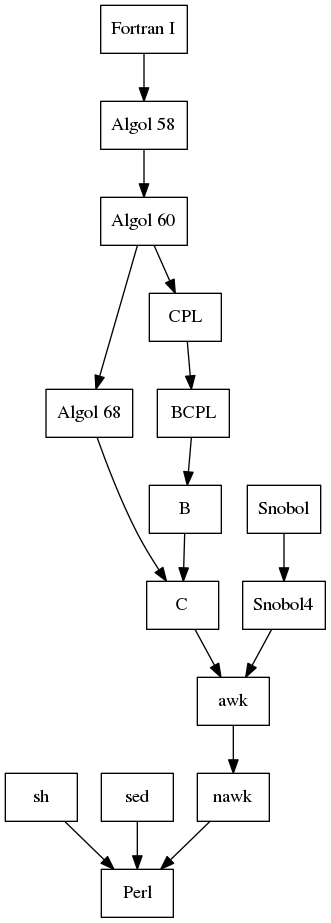
\includegraphics[height=0.5\textheight]{perl}
  \captionof{figure}{Inheritance diagram for \cd{Perl}.}
\end{Figure}

\newpage
\end{document}
